%Dokumentenklasse "scrbook" - Erweitert um den Verweis auf die Verzeichnisse und Texteigenschaften
\documentclass[chapterprefix=true, 12pt, a4paper, oneside, parskip=half, listof=totoc, bibliography=totoc, numbers=noendperiod]{scrbook}

% Ränder (Standard bottom ca. 52mm anbzüglich von ca. 4mm für die nach oben rechts gewanderte Seitenzahl)
%Anpassung der Seitenränder
\usepackage[bottom=48mm,left=25mm,right=25mm]{geometry}

% Ränder bei Bedarf zeigen
%\usepackage{showframe}

%Tweaks für scrbook
\usepackage{scrhack}

%Blindtext
\usepackage{blindtext}

%Erlaubt unteranderem Umbrücke captions
\usepackage{caption}

%Stichwortverzeichnis
\usepackage{imakeidx}

%Kompakte Listen
\usepackage{paralist}

%Zitate besser formatieren und darstellen
\usepackage{epigraph}

%Glossar, Stichworverzeichnis
\usepackage[toc, acronym]{glossaries} % Akronyme werden als eigene Liste aufgeführt

%Anpassung von Kopf- und Fußzeile
%beinflusst die erste Seite des Kapitels
\usepackage[automark,headsepline]{scrlayer-scrpage}
\automark{chapter}
\ihead{\leftmark}
\chead{}
\ohead{\thepage}
\ifoot*{}
\cfoot[\thepage]{}
\cfoot*{}
\ofoot*{}
\pagestyle{scrheadings}

%Auskommentieren für die Verkleinerung des vertikalen Abstandes eines neuen Kapitels
%\renewcommand*{\chapterheadstartvskip}{\vspace*{.25\baselineskip}}

%Zeilenabstand 1,5
\usepackage[onehalfspacing]{setspace}

%Verbesserte Darstellung der Buchstaben zueinander
\usepackage[stretch=10]{microtype}

%Deutsche Bezeichnungen für angezeigte Namen (z.B. Innhaltsverzeichnis etc.)
\usepackage[ngerman]{babel}

%Unterstützung von Umlauten und anderen Sonderzeichen (UTF-8)
\usepackage{lmodern}
\usepackage[utf8]{luainputenc}
\usepackage[T1]{fontenc}

%Einfachere Zitate
\usepackage{epigraph}

%Verwendung von Akronymen
\usepackage[printonlyused]{acronym}

%Unterstützung der H positionierung (keine automatische Verschiebung eingefügter Elemente)
\usepackage{float} 

%Erlaubt Umbrüche innerhalb von Tabellen
\usepackage{tabularx}

%Erlaubt Seitenumbrüche mit Tabellen
\usepackage{longtable}

%Erlaubt die Darstellung von Sourcecode mit Highlighting
\usepackage{listings}

%Definierung eigener Farben bei nutzung eines selbst vergebene Namens
\usepackage[table,xcdraw]{xcolor}

%Vektorgrafiken
\usepackage{tikz}

%Grafiken (wie jpg, png, etc.)
\usepackage{graphicx}

%Grafiken von Text umlaufen lassen
\usepackage{wrapfig}

%Ermöglicht Verknüpfungen innerhalb des Dokumentes (e.g. for PDF), Links werden durch "hidelink" nicht explizit hervorgehoben
\usepackage[hidelinks,german]{hyperref}
\usepackage{nameref}
%Einbindung und Verwaltung von Literaturverzeichnissen
\usepackage{csquotes} %wird von biber benötigt
\usepackage[style=alphabetic,citestyle=alphabetic,backend=biber,bibencoding=UTF-8]{biblatex}
\addbibresource{references/references.bib}
\nocite{*}
%-------------------------------Zusätzliche Anpassungen und Modifikationen--------------------------------------------%

%Anpassung der Überschriften
\addtokomafont{disposition}{\rmfamily}

%Zusätzliche Farben
\definecolor{darkgreen}{RGB}{0,100,0}

%Umbenennungen
\renewcommand{\lstlistlistingname}{Quelltextverzeichnis}

%Pluszeichen in der Referenc beim zitieren ausblenden
\renewcommand*{\labelalphaothers}{}

%Anpassugen zur Quelltextdarstellung, kann bei Bedarf überschrieben werden (z.B. wenn unterschiedliche Sprachen zum Einsatz kommen)
\renewcommand{\lstlistingname}{Codeauszug}
\lstset{
	language=Java,
	numbers=left,
	columns=fullflexible,
	aboveskip=5pt,
	belowskip=10pt,
	basicstyle=\small\ttfamily,
	backgroundcolor=\color{black!5},
	commentstyle=\color{darkgreen},
	keywordstyle=\color{blue},
	stringstyle=\color{gray},
	showspaces=false,
	showstringspaces=false,
	showtabs=false,
	xleftmargin=16pt,
	xrightmargin=0pt,
	framesep=5pt,
	framerule=3pt,
	frame=leftline,
	rulecolor=\color{green},
	tabsize=2,
	breaklines=true,
	breakatwhitespace=true,
	prebreak={\mbox{$\hookleftarrow$}}
}

%Anpassungen für das Abkürzungsverzeichnis
\newglossarystyle{dottedlocations}{%
	\glossarystyle{list}%
	\renewcommand*{\glossaryentryfield}[5]{%
		\item[\glsentryitem{##1}\glstarget{##1}{##2}] \emph{##3}%
		\unskip\leaders\hbox to 2.9mm{\hss.}\hfill##5}%
	\renewcommand*{\glsgroupskip}{}%
}

%%Titles - Uncomment one section of titles

%%Used for titleGraduation
\include{titles/titleGraduation}
\logoPathL{} %just leave empty to hide logo
\logoWidthL{0.5}
\logoPathR{resources/HTW_Berlin_Logo_pos_GRAU_RGB.jpg} %just leave empty to hide logo
\logoWidthR{1}
\gradeType{Master of Science (M.Sc.)}
\secondExaminer{Max Mustermann}

%%Used for titleResearchPaper
%\makeatletter

\newcommand*{\firstExaminer}[1]{\gdef\@firstExaminer{#1}}
\newcommand*{\subTitle}[1]{\gdef\@subTitle{#1}}
\newcommand*{\researchPart}[1]{\gdef\@researchPart{#1}}
\newcommand*{\matrikelnr}[1]{\gdef\@matrikelnr{#1}}
\newcommand*{\submitDate}[1]{\gdef\@submitDate{#1}}


\renewcommand*{\maketitle}{
	\begin{titlepage}
		\newgeometry{left=2.5cm,right=2.5cm,top=9.0cm,bottom=2.5cm}
		\begin{center}
			\vfill
			{\Large \@title\par}
			{\normalsize \@subTitle\par}
			\vskip 0.5cm
			{\large an der}
			\vskip 0.5cm
			{\large Humboldt-Universität zu Berlin\\ Studiengang Informatik (M.Sc.)}
			\vfill
			\begin{flushleft}
				\begin{tabular}[t]{rl}
					Authoren: &\@author\\
					\ifx\@matrikelnr\empty
					\else
					Matrikelnummer: & \@matrikelnr\\
					\fi
					Datum der Abgabe: & \@submitDate
				\end{tabular}
			\end{flushleft}
		\end{center}
		\restoregeometry
	\end{titlepage}
}
\makeatother
%\subTitle{Ein optionaler Untertitel der Arbeit}
%\researchPart{A}

%%Used by all titles
\title{Dies ist der Titel der Abschlussarbeit der sich auch über mehrere Zeilen erstrecken kann}
\author{Max Mustermann}
\matrikelnr{s0000000} % just leave empty to hide number
\submitDate{05.10.2015}
\firstExaminer{Max Mustermann}
%%End Titles

\makeindex[title=Stichwortverzeichnis, options=-s indexstyle.ist, intoc]
\indexsetup{level=\chapter*,toclevel=chapter}


\makeglossaries
\loadglsentries{glossary_and_acronyms.tex}
\setacronymstyle{long-short}

\begin{document}

\pagenumbering{alph} %fix for same identifier warning, character is not show in title
\maketitle

\pagenumbering{Roman}

\chapter*{Abstract}
Algorithmen und Computer bestimmen immer häufiger Entscheidungen in unserem Leben. Aber es ist auffällig, dass diese nicht immer so neutrale Ergebnisse liefern, wie man es erwarten würde.
\newline
In dieser Arbeit werden verschieden Anhaltspunkte aufgezeigt, die dafür sprechen, dass ein Algorithmus verzerrte Ergebnisse liefern kann. Außerdem werden einige Beispiele genannt. \clearpage
% Eigenständigkeitserklärung
\chapter*{Eigenständigkeitserklärung}

Hiermit versichere wir, dass wir die vorliegende Masterarbeit selbstständig und nur unter
Verwendung der angegebenen Quellen und Hilfsmittel verfasst haben. Die Arbeit wurde bisher
in gleicher oder ähnlicher Form keiner anderen Prüfungsbehörde vorgelegt.

\vskip 1cm

Berlin, den \today

\vskip 1.5cm

Alena Schemmert und Lukas Jünemann \clearpage

\tableofcontents \newpage

\pagenumbering{arabic}
\chapter{Einleitung}

Im Rahmen des Seminars \enquote{Ethische Fragen der Informatik} an der Humboldt-Universität zu Berlin, sollte sich der Kurs mit verschiedenen aktuellen Themen auseinandersetzen. Diese Gruppe hat einen Vortrag zu sogenannten 'Biased Algorithems' ausgearbeitet, der im Nachfolgenden nochmals verschriftlich wurde.

\section{Motivation}

Aufgrund von häufigeren Berichten in Onlinemagazinen und Social-Media-Plattformen, wird das Thema \enquote{Biased Algorithmens} immer präsenter in unserer Gesellschaft. Vor Allem, da Algorithmen immer mehr Probleme in unserem Alltag lösen und somit einen zunhemend größeren Einfluss auf unser soziales Leben nehmen.
Gerade als Student-in der Informatik stellt sich einem die Frage, welche Verantwortung man selbst im späteren Berufsleben beim Entwickeln von Software hat. Es stellt sich also die Frage, was ist ein \enquote{Biased Algorithm} und wie kann man dies bei der Entwicklung vermeiden.



\section{Begriffserklärung}


\subsection{Algorithmus}
Da es verschiedene Definitionen des Wortes Algorithmus gibt, wurde der Versuch unternommen im Rahmen dieser Ausarbeitung lediglich Kriterien zu benennen die einen Algorithmus im Sinne des Themas von anderen Begriffen wie Software, Framework oder künstlicher Intelligenz unterscheiden. Dabei wurden 5 Kriterien festgelegt:
\begin{itemize}
	\item Maschinenlesbarkeit / Maschinenausführbarkeit
	\item Lösung eines konkreten Problems
	\item Berstehend aus einer endlichen Menge an Anweisungen
	\item Endliche Verarbeitungszeit
	\item Gleiche Eingabe erzeugt gleiche Ausgabe
\end{itemize}
Insbesondere das letzte Kriterium wurde gewählt um sich bewusst von Thema künstlicher Intelligenz abzusetzen.

% * <Alena Schemmert> 17:05:29 23 Sep 2019 UTC+0200:
% Noch offen
\subsection{Biased Algorithm}
\enquote{Biased} ist ein englisches Wort, für welches es viele Übersetzungen gibt. Dazu gehören Verzerrt, Parteiisch, Voreingenommen, Tendenziös, Uneinheitlich. Die treffendste Übersetzung ist verzerrt, da parteiisch, voreingenommen oder tendenziös einem Algorithmus unterstellen würden, er hätte eine eigne Meinung. Uneinheitlich widerspricht der allgemeinen Definition eines Algorithmus, da dieser ja deterministisch sein soll.  
 \clearpage
\chapter{Ethische Bedenken bei Algorithmen}

\section{Allgemeine Bedenken}

\begin{figure}
  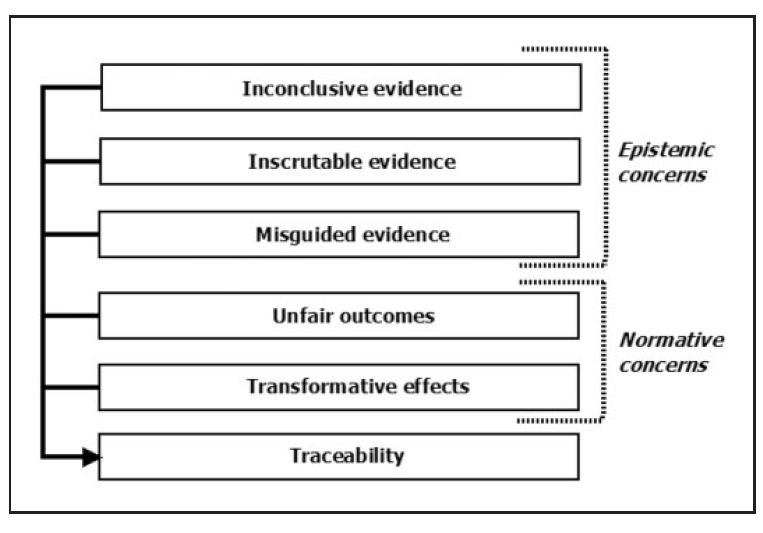
\includegraphics[width=\linewidth]{resources/ethical_concerns.png}
  \caption{Six types of ethical concerns raised by algorithms, (S. 4, Figure 1 )}
  \label{fig:Ethische Bedenken}
\end{figure}


% * <Alena Schemmert> 17:06:07 23 Sep 2019 UTC+0200:
% Hier fehlt noch eine Beschreibung zum Bild

\subsection{Uneindeutige Anhaltspunkte}
 Künstliche Intelligenzen und allgemein Algorithmen des machinellen Lernens ziehen viele Schlussfolgerungen auf Grundlage von Wahrscheinlichkeiten und statistischen Mitteln.
 Deshalb sind die Ergebnisse zwar überprüfbar, aber mit Unsicherheit versehen.
 Das ist auch problematisch da häufig statistische Korrelationen benutzt werden. Aber Korrelation ist nihct gleich Kausalität - nur weil zwei Sachen immer im gleichen Kontext auftaucht, bedingen diese sich nicht gegenseitig.
 Häufig wird solche Software in einem Kontext eingesetzt in der zuverlässige Techniken und Daten entweder nicht verfügbar sind, oder zu aufwändig zu implementieren wäre. Dies sollte beachtet werden, wenn aus den Ergebnissen von Algorithmen Erkenntnisse gewonnen werden sollen. 


\subsection{Undurchsichtige Anhaltspunkte}

 Als zweiten Faktor neben statistischen Mitteln, die die Ergebnisse von Algorithmen verzerren, werden in dem Paper Parameter genannt. Die Parameter eines Algorithmus können ebenfalls die Wahrscheinlichkeiten von einem Ergebnis beeinflussen. Ein großes Problem hierbei ist, dass der Zusammenhang zwischen Daten und Ergebnis häufig nicht öffentlich zugänglich. Hilfreich wäre die Zusammenhänge zwischen einzelnen Daten, sowie Parametern und deren Ergebnissen in einer Erklärung zu veröffentlichen. Allerdings ist die Funktionalität eines Algorithmus meistens ein Geschäftsgeheimnis, da man diese nicht erklären kann, ohne den Algorithmus selbst zu veröffentlichen. 
 Dies liegt in der Natur der Sache: Algorithmen sind die Beschreibung zur Abarbeitung einer Teilaufgabe. Also, wie soll man dir Beschreibung beschreiben, ohne zu viel zu verraten, aber gleichzeitig genug, um Vetrauen zu schaffen? 
 Sozusagen entstehen ethische Bedenken, wenn Algorithmen in eine BlackBox agieren. 
 

\subsection{Fehlgeleitete Anhaltspunkte}

\subsection{Unfaire Ergebnisse}

Die vorherigen drei Bedenken beschäftigten sich mit dem Erkenntnisgewinn eines Algorithmus. Die ethischen Bedenken können jedoch auch erst beim Resultat entstehen. Vor allem dann, wenn Handlungen auf ein Ergebnis eines Algorithmus folgen, können diese ethisch unterschiedlich bewertet werden. Diese Bewertung kann man unter dem Wort "Fairness" zusammenfassen. 
So kann ein Ergebnis von einer diskriminierten Gruppe als unfair betrachtet werden, allein weil eine andere Klasse von Menschen bevorteilt wird. 
Als ein Beispiel für (un)faire Handlung aufgrund von Ergebnissen von Algorithmen, sind Vorschläge zu Berechnung von Krankenkassenbeiträge. Die erste Variante schlägt vor, dass Mitglieder mit schlechten Gesundheitswerten und wenig Eigeninitiative mehr als den Grundsatz bezahlen. Die andere Variante hingegen, dass Mitglieder mit guten Gesundheitswerten und viel Eigeninitiative einen Rabatt bekommen. 
Die Umfrage während des Vortrages hat ergeben, dass die zweite Variante höchstwahrscheinlich beer akzeptiert wird, auch wenn diese Variante als ebenfalls unfair betrachtet werden können.


\subsection{Transformative Effekte}

% * <Alena Schemmert> 17:06:27 23 Sep 2019 UTC+0200:
% Muss noch geschrieben werden

\subsection{Nachverfolgbarkeit}

% * <Alena Schemmert> 17:06:32 23 Sep 2019 UTC+0200:
% Muss noch geschrieben werden

\section{Verzerrte Algorithmen}

Verzerrte Algorithmen lassen sich in drei soziale Problemfelder einteilen, da nicht alle unfairen Ergebnisse eines Algorithmus den gleichen Einfluss auf unser Leben haben. 
Diese sind Entscheidungsalgorithmen, Empfehlungsalgorithmen, wie Kaufempfehlungen und Life-Style-Software.


\subsection{Entscheidungsalgorithmen}
Unter Entscheidungsalgorithmen versteht man die automatisierte Entscheidung über beispielsweise die Vergabe eine Kredites durch einen Algorithmus. In diesem Bereich gibt es einige Beispiele von verzerrte Algorithmen. 

\subsubsection{SCHUFA}
Die SCHUFA (Schutzgemeinschaft für allgemeine Kreditsicherung, Wiesbaden) ist ein Unternhemen, welches für Personen einen Score berechnet um die Kreditwürdigkeit abzubilden. Dieser Score wird anhand von verschiedenen Parametern bestimmt. Neben bereits existierenden Krediten oder Anzahl der Kontenüberziehung wird ebenfalls der Wohnort der Person in die Berechnung mit einbezogen. \newline

“Rein statistisch ist es tatsächlich unwahrscheinlicher, von jemandem, der in einem 150-Parteien-Hochhaus mit vielen Schuldnern lebt, einen Kredit zurückzubekommen“
[Thomas Riemann, Welt, 20.05.15 Geschäftsführer “Verband der Wirtschaftsauskunfteien”]

In vielen Fällen kann es dazu führen, dass der Score schlechter ausfällt, da er auch von statistischen Mitteln abhängt. \cite{welt2015}


Die Analyse einer Person anhand Ihrer Umgebung und Eigenheiten nennt man Profiling. 

\subsection{Profiling}


% * <Alena Schemmert> 17:04:37 23 Sep 2019 UTC+0200:
% Muss Noch richtig geschrieben werden
Profiling Algorithmen erkennen Korrelationen
- Und machen Vorhersagen über Verhalten auf Gruppen-Ebene

- Personen werden anhand von Verbindungen zu anderen Personen verglichen
- Anstatt das tatsächliche Verhalten von Individuen zu bewerten

- Der Handlungsrahmen einer Person wird anhand von Informationen zur Personen-Gruppe abgesteckt
- Es ist deshalb sehr naheliegend, dass diese Art von Algorithmen zu Diskriminierung neigen

- Daten-basierte Diskriminierung ist genauso wenig zu ertragen wie soziale Diskriminierung aufgrund von Vorurteilen
- Diskriminierung ist das Ergebnis wiederholter Verzerrung
- Und fördern damit Schubladen-Denken 

\subsection{Empfehlungsalgorithmen}

% * <Alena Schemmert> 17:07:27 23 Sep 2019 UTC+0200:
% Muss noch geschrieben werden

\subsection{Life-Style-Software}

Unter Life-Style-Software verstehen wir Technologien, die uns das Leben vereinfachen sollen. Aber auch hier kann das Gegenteil eintreten, wenn die Software nicht immer wie angepriesen funktioniert. 
Ein Beispiel dafür ist ein Seifenspender welcher mit einer Künstlichen Intelligenz ausgestattet wurde. Dieser steht angeblich im Facebook Hauptbüro. 
Der Seifenspender soll automatisch Hände erkennen und eine gewissen Menge Seife in die Hände geben. Allerdings erkennt dieser Seifenspender keine dunkelhäutigen Hände. \newline 

Ein anderes Gadget welches eiegentlich das Leben erleichtern soll, aber doch häufig zu einem Ärgernis werden, ist die Fitness-Tracker-App von fitbit. Die App soll einem helfen, die eigene Aktivität oder Schlafzyklen zu messen. Zusätzlich kann man die eigene Kalorienaufnahme und das eigene Gewicht mitverfolgen. Da die täglich nötige Kalorienzufuhr und Bewegung abhängig von der physischen Verfassung ist, kommt es zu einem Problem. Vor allem bei schwangeren Frauen ist eine Gewichtszunhame und eine höhere Kalorienzufuhr wichtig für die Gesundheit. Zum Ende der Schwangerschaft, nimmt die Bewegung ab. Durch die App werden diese Aktivitäten negativ bewertet, da sie darauf programmiert ist, hohe AKtivität und vermeintlich gesundes Leben mit positiven Nachrichten zu belohnen. 
Als Frau kann man in der App einstellen, wann die Regelblutung normalerweise eintritt, oder welches Verhütungsmittel genutzt wird, aber nicht, dass man zurzeit schwanger ist und somit die anstehenden Veränderungen normal und gesund sind. 
Aber anstatt dessen, werden Frauen in besonderen Umständen mit Pushnachrichten dazu angehalten, sich mehr zu bewegen um wieder abzuspecken. 
Dieses Feature wird sich seit 2008 von der Nutzer-Community immer wieder gewünscht und betrifft immerhin die Hälfte aller potenziellen Kunden. 


\subsection[feature]{Diskussion - Ist Verzerrung eine Frage mangelnder Features?}

% * <Alena Schemmert> 17:13:23 23 Sep 2019 UTC+0200:
% Muss noch geschrieben werden. Notizen aus Vortrag
 \clearpage
\chapter{Zusammenfassung}

\section{Fazit}

\section{Ausblick}


 \clearpage

% Anhang
\chapter*{Quellen}
\pagenumbering{Alph}
\printbibliography[heading=bibintoc, keyword={book}, title={Literaturverzeichnis}]\clearpage
\printbibliography[heading=bibintoc, keyword={online}, title={Onlinequellen}]\clearpage
\printbibliography[heading=bibintoc, keyword={image}, title={Bildquellen}]\clearpage

\chapter*{Anhang}
\printglossary[style=dottedlocations,type=\acronymtype,title={Abkürzungsverzeichnis}] \clearpage

\listoffigures \clearpage

\printindex \clearpage

\end{document}